%\documentclass[11pt,a4paper,roman]{moderncv}
\documentclass[a4paper,titlepage]{article}
\usepackage[scale=.85]{geometry}
\usepackage{graphicx}
\usepackage{wrapfig}
\pagenumbering{gobble}
%\moderncvstyle{classic}

%\firstname{Kyle}
%\familyname{Hershey}
%\address{2296 Long Avenue}{Saint Paul, MN 55114}
%\phone{608 345 8595}
%\email{hersh029@umn.edu}

\begin{document}
\Huge \noindent KYLE W. HERSHEY \hfill 
\footnotesize \parbox[b]{2in}{\begingroup \raggedleft2296 Long Avenue\\Saint Paul, MN 55114\\(608)-345-8595\\hersh029@umn.edu \par \endgroup}
%\small \parbox[b]{2in}{2296 Long Avenue\\Saint Paul, MN 55114\\608 345 8595\\hersh029@umn.edu}
%\makecvtitle
\normalsize
\vspace{1ex}
\hrule
\vspace{-2ex}

\section*{Overall Research Summary}
My doctoral work with Professor Russell Holmes at the University of Minnesota has focused on understanding kinetic processes within Organic Light-Emitting Devices (OLEDs).  Emission of light from OLEDs requires efficient formation and recombination of molecular excited states, called excitons.  Understanding the mechanisms that limit the efficiency of these processes provides an opportunity to increase the overall efficiency, brightness and lifetime of devices.

Work on understanding these kinetic processes was conducted in the transient  (on the order of microseconds), steady-state, and operational lifetime regimes.  My work has focused on two main goals:

\begin{itemize}
\item Unifying the transient and steady-state behavior of OLEDs under a single kinetic model
\item Decoupling degradation pathways during operational lifetime testing of OLEDs
\end{itemize}

\section*{Unifying Transient and Steady-State Behavior}

Under steady-state excitation, OLEDs show a decrease in efficiency with increasing current and brightness, known as the efficiency roll-off.  This has been previously attributed to bimolecular quenching processes involving excitons and charges.  However, the mean field differential equations models used to replicate this behavior are not capable of predicting the transient behavior and thus offer an incomplete picture.  

\begin{wrapfigure}{r}{0.4\textwidth}
\vspace{-15pt}
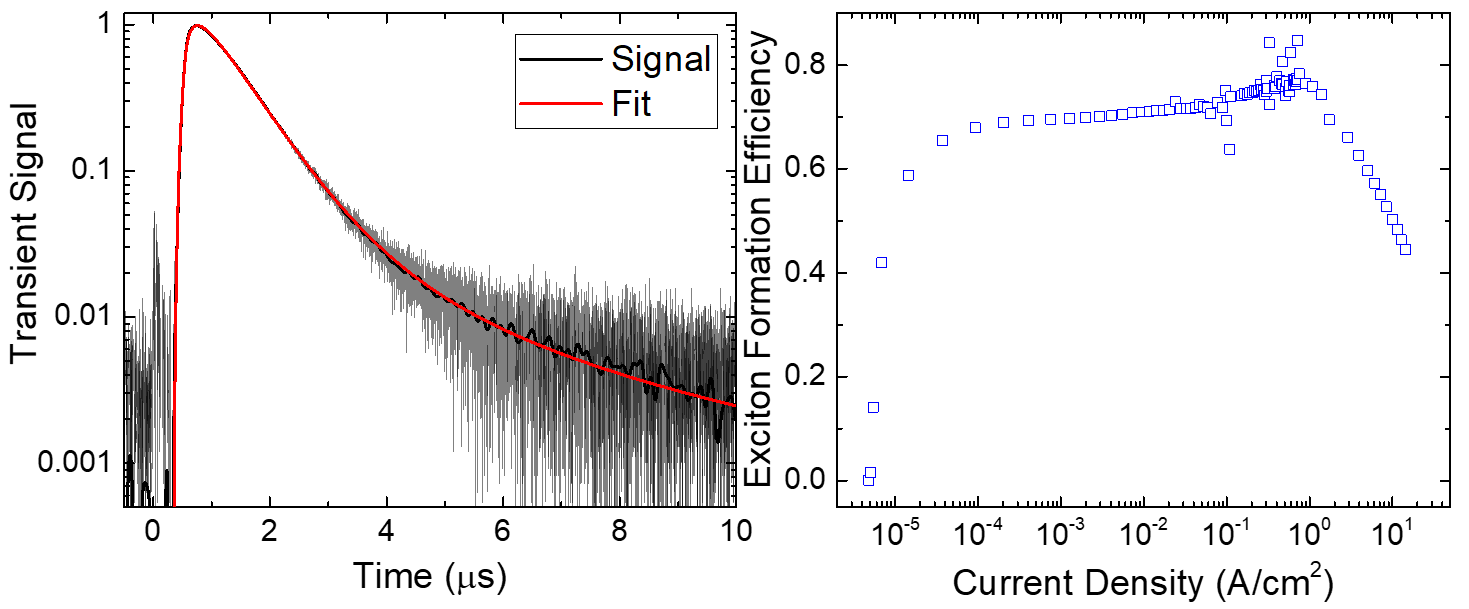
\includegraphics[width=0.4\textwidth]{unified}
\vspace{-20pt}
\end{wrapfigure}

Using the green emitter, Tris[2-phenylpyridinato-C\textsuperscript{2},N]iridium(III) (Ir(ppy)\textsubscript{3}), I expanded upon the existing model by including charge dynamics.  In my model, upon the application of current, charges are injected into the device and can either form excitons or leak through the device.  With these added kinetics, the transient behavior and the current dependence of the steady-state efficiency were able to be fit simultaneously with the same model and rate constants.  The transient behavior was able to be fit as a function of voltage and an example fit is shown in the left panel of the figure.  

In previous works, only the efficiency roll-off was replicated with the dynamics model.  With the inclusion of charge dynamics, I was able to fit both the rise and fall of efficiency which had not been previously done.  Additionally, defining dynamics allowed for a rigorous definition of exciton formation efficiency, which I was able to extract, shown in the right panel.  The charge leakage time through the device, which I introduced, was consistent with a drift model using known charge mobilities.  The extracted model parameters were all able to be independently verified, with the except for the exciton formation rate, leaving only one free parameter required to explain both regimes.

\section*{Decoupling Degradation Pathways During Operational Lifetime}

OLED lifetime is difficult to optimize due to the time required to measure and the minimal information acquired from traditional measurements which record luminance loss over time at a fixed current density.  In order to accelerate optimization, a better understanding of the loss pathways is required.  

\begin{wrapfigure}{r}{0.25\textwidth}
\vspace{-15pt}
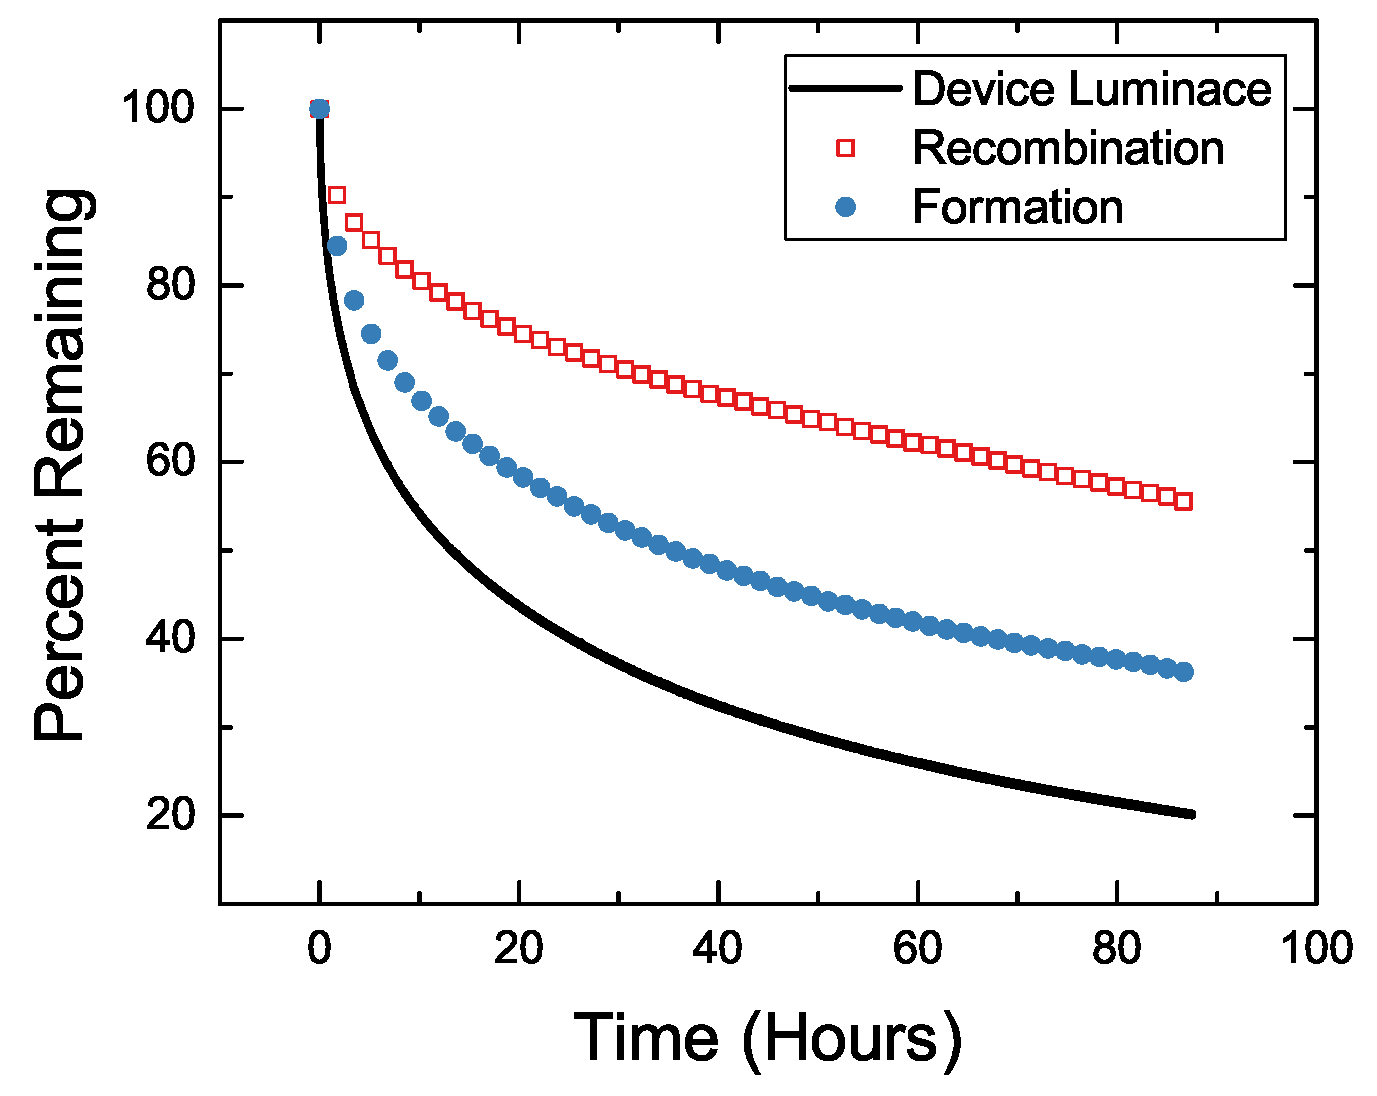
\includegraphics[width=0.25\textwidth]{lifetime}
\vspace{-20pt}
\end{wrapfigure}

In an effort to address this problem, I have classified luminance loss overtime into two categories:  exciton formation and recombination efficiency losses.  To extract these quantities, I have developed a measurement technique involving traditional constant current excitation with periodic optical excitation using a laser to measure the recombination efficiency.  This has involved both hardware and software development to create a novel lab measurement apparatus.  While not changing the lifetime results of the original test, this technique is able to isolate exciton formation losses from recombination losses, shown in the figure.  This information can be helpful in determining degradation mechanisms and presenting possible means of improvement.

Using a single device architecture with three different emissive layer thicknesses, I was able to show that for this architecture, exciton formation efficiency loss was limiting the lifetime and for thin emissive layers, was being accelerated by exciton formation at a layer interface.  The use of this technique enables the easy determination of these limiting rates and will help in identifying degradation mechanisms, accelerating device optimization.

\end{document}
